
\begin{comment}
    parti fa chiarire con Matarrese

    - non mi torna la definizione di R_tau
    - che significato ha la condizione iniziale xi = -1 + q^3/6...
    - come si posizionano i tempi tau comin e comax rispetto alla linea temporale, o rispetto a tau = 1?
        sono entrambi dopo l'istante tau = 1, perchè sono in shell crossing credo


\end{comment}



\section{Setup e scelta delle condizioni iniziali}

In cosmologia le caustiche, che nascono da una singolarità nella trattazione di fluido esposta nel precedente
capitolo, rappresentano in realtà il processo fondamentale della formazione di strutture a grande scala 
nell'universo. Al primo shell-crossing le particelle affrontano il \textit{collasso gravitazionale
secondario}, per cui il numero di collisioni aumenta sostanzialmente, e così aumenta il numero di pancakes e 
strutture filiformi. Tuttavia la forma oblata quasi unidimensionale del pancake non è l'unica forma che si 
registra: infatti nel contesto di una trattazione nonlineare della dinamica gravitazionale con l'approssimazione
di Zel'dovich si incontrano una serie di strutture scrupolosamente classificate per i casi semplici unidimensionale
e bidimensionale in \cite{arnold}.

Tuttavia la varietà di strutture che può emergere a seguito del collasso gravitazionale non possono essere previste 
da un modello che include l'approssimazione di Zel'dovich, la quale si basa sull'ipotesi di velocità costante.
In effetti si è spiegato nel primo capitolo che ZA risulta essere una soluzione esatta solamente nel caso 
unidimensionale, e in ogni caso valida esclusivamente fino al primo shell-crossing, dove le equazioni del
fluido falliscono. \'E necessario quindi tornare all'equazione di riferimento, ossia all'equazione di Vlasov 
\ref{eqn:vlasov}, anche limitandosi in prima battuta al caso unidimensionale, dal momento che gli 
shell-crossing si manifestano, almeno nella loro fase iniziale, come fenomeni unidimensionali.

Inquadriamo l'analisi in un universo EdS, dove $\tau = a$ come accennato in precedenza, quando abbiamo anche
fornito la definizione $u(x(q, \tau), \tau) = \partial_a x(q, \tau) = \partial_{\tau}(q, \tau) = \dot{x}(q, \tau)$.
Si riportano le equazioni \ref{eqn:cont_tau} e \ref{eqn:poisson_tau}.

\begin{gather}
    \label{eqn:cont_new}
    \ddot{x} + \frac{3}{2\tau}\dot{x} = - \frac{3}{2\tau}\nabla_x \phi \\
    \label{eqn:poisson_new}
    \laplacian_x\phi = \frac{\delta}{\tau}
\end{gather}
dove si ricorda che $\delta = (\rho - \rho_b)/\rho_b$ rappresenta la deviazione dalla densità media, e sia $\delta$
che $\phi$ dipendono da x. In particolare si può riscrivere 
\begin{equation}
    \label{eqn:density}
    \delta(x(q, \tau), \tau) = \int dq' \delta_D[x(q, \tau)-x(q', \tau)] - 1
\end{equation}
dove $\delta_D$ è una delta di Dirac che dà contributo quando due particelle partite da diverse
posizioni iniziali $q$ e $q'$ collidono nella stessa posizione euleriana $x$.

Si osserva ora che tale set di equazioni gode di invarianza rispetto a trasformazioni di 
Galileo della forma $x \mapsto x + \zeta(\tau)$: possiamo sfruttare al presenza di questa 
simmetria per imporre una condizione al centro di massa. Per scriverla definiamo il dislocamento
lagrangiano $\xi(q, \tau):= x(q, \tau) - q$.

\begin{equation}
    \label{eqn:com}
    \int_{\mathbb{T}}\xi(q', \tau) dq' = 0
\end{equation}
Se tale condizione non fosse rispettata significherebbe che esiste un certa direzione
privilegiata di moto delle particelle, incompatibilmente con l'assenza di forze esterne.

A questo punto si procede prendendo la divergenza di \ref{eqn:cont_new} e inserendovi 
\ref{eqn:poisson_new}, ottenendo

\begin{equation}
    \nabla_x \ddot{x} + \nabla_x \left(\frac{3}{2\tau}\dot{x}\right) = -\frac{3}{2\tau}\laplacian_x\phi = -\frac{3\delta(x)}{2\tau^2}
\end{equation}
Sostituendo $\nabla_x = \partial_x q \nabla_q$, si ottiene

\begin{gather}
    \nabla_q \ddot{x} + \frac{3}{2\tau} \nabla_q\dot{x} = -\frac{3}{2\tau^2}\frac{\partial x}{\partial q}\delta(x(q,\tau)) \\
    \label{eqn:progress}
    \nabla_q \left[ \tau^2 \partial^2_{\tau} + \frac{3}{2}\tau \partial_{\tau} \right] x = -\frac{3}{2}\frac{\partial x}{\partial q}\delta(x(q,\tau))
\end{gather}
A questo punto definiamo la funzione $F(x(q, \tau))$ come una forza "efficace" di multistreaming, utilizzando 
la definizione della densità \ref{eqn:density}. Nel dettaglio, $F(x(q, \tau)) = (\partial_q x) \int \delta_D[x(q, \tau)-x(q', \tau)]dq' -1$.
Ma allora il secondo membro della \ref{eqn:progress} si può scrivere come

\begin{equation}
    -\frac{3}{2} (\partial_q x )\delta = -\frac{3}{2}(F+1-\partial_q x) = -\frac{3}{2} F +\frac{3}{2} (\partial_q x - 1) = -\frac{3}{2} F + \frac{3}{2} \partial_q \xi    
\end{equation}
dato che in effetti $\partial_q \xi = \partial_q (x-q) = \partial_q x - 1$. 

Il primo membro di \ref{eqn:progress} invece contiene un operatore temporale che agisce su $x$. Se si scrive $x(q,\tau) = \xi(q, \tau) + q$ e si nota che q non 
dipende dal tempo, è equivalente far agire l'operatore su $\xi$ anzichè su x. 

\begin{gather}
    \partial_q \left[ \tau^2 \partial^2_{\tau}+\frac{3}{2}\tau\partial_{\tau} \right] \xi = -\frac{3}{2}F(x(q,\tau)) +\frac{3}{2}\partial_q \xi \\
    \label{eqn:Fequation}
    \partial_q \mathcal{R}_{\tau}\xi = -\frac{3}{2}F(x(q, \tau))
\end{gather}
dove si è definito l'operatore $\mathcal{R}_{\tau} = \tau^2\partial^2_{\tau} + (3\tau/2)\partial\tau-3/2$.
Integrando ora la \ref{eqn:Fequation} sulla coordinata $q$, sarà possibile ottenere l'equazione 
del moto del dislocamento $\xi$.

\begin{equation}
    \label{eqn:Sequation}
    \mathcal{R}_{\tau}[\xi(q, \tau)-\xi_c(\tau)] = -\frac{3}{2}S(x(q, \tau))
\end{equation}
dove $S$ è definito come l'integrale della forza generalizzata $S = \int_0^q F(q',\tau)dq'$ e $\xi_c$ rappresenta il 
dislocamento alla coordinata $q=0$.
Per potere risolvere l'equazione differenziale espressa nella \ref{eqn:Sequation} ci occorrono
però delle condizioni iniziali per l'istante $\tau = 0$.

\begin{equation}
    \label{eqn:initcond}
    \xi(q, 0) = -q + \frac{q^3}{6} + cq^4 + o(q^4) = \xi_{ZA}^{ini}
\end{equation}
in cui si assume c<\!<1. Questa condizione iniziale viene da \cite{zeldovich}, in cui si applica
un'espansione di Taylor al potenziale gravitazionale, sapendo che quest'ultimo, nell'approssimazione di Zel'dovich, 
esatta in una dimensione, è collegato alla velocità, come evidente in \ref{eqn:zelsol}, dove si osserva che la 
velocità non è altro che la derivata del potenziale. Proviamo dunque a espandere il potenziale

\begin{gather}
    \label{eqn:phiexp}
    \phi(q) = \phi_0 + a_1 q + a_2 q^2 + a_3 q^3 + o(q^3) \\
    \phi'(q) = a_1 + 2 a_2 q + 3 a_3 q^2 + o(q^2) \\
    \phi''(q) = 2a_2 +6a_3 q + o(q) \\
    \phi'''(q) = 6a_3 + o(const) 
\end{gather}
La derivata seconda del potenziale è tuttavia esprimibile tramite gli autovalori $\lambda(q)$ del tensore di deformazione,
come mostrato nel capitolo precedente. Pertanto, nel momento in cui si adotta l'ipotesi di minimo per tale autovalore,
ossia per la derivata seconda del potenziale, si chiede $\lambda'(q)=0$, cioè $\phi'''(q)=0$. Pertanto è conveniente la
scelta $a_3 = 0$, che priva la derivata prima $\phi'(q)$, e con essa la velocità, della terza potenza.
L'espansione proposta in \ref{eqn:phiexp} è quella proposta in \cite{colombi}, mentre in \cite{rampf} si 
raggiungono gradi superiori arrivando a disporre del termine di quarto grado nella velocità, come espresso in \ref{eqn:initcond}.

Finchè non vi sono eventi di collisione, ossia nella regione di single-stream, non si verificano 
sovrapposizioni tra coordinate euleriane generate da diversi antecedenti lagrangiani, ossia $x(q)\neq x'(q')$.
Questo rende l'espressione di densità \ref{eqn:density} nulla, e con essa anche la forza generalizzata
$F(x(q, \tau)$ e il suo integrale $S(x(q, \tau)$. Pertanto l'equazione \ref{eqn:Sequation} si riduce
a $\mathcal{R}_{\tau}[\xi(q, \tau)-\xi_c(\tau)] = 0$. Sfruttando inoltre la condizione del centro di 
massa \ref{eqn:com}, imponiamo $\xi_c = 0$, recuperando così la soluzione di Zel'dovich.

\begin{equation}
    x_{ZA}(q, \tau) = q+ \tau \xi_{ZA}^{ini}
\end{equation}
Sappiamo che tale soluzione risulta valida solamente fino al primo shell-crossing, momento in cui si verifica
la condizione $\partial_q x_{ZA} = 0$, che causa invece la divergenza della densità prima nulla.
Infatti, ricordando la proprietà della delta di Dirac

\begin{equation}
    \label{eqn:dirac}
    \delta_D(f(x)) = \sum_i \frac{\delta_D(x-a_i)}{f'(a_i)}
\end{equation}
dove $\{a_i\}$ sono gli zeri di $f(x)$, si trova che la \ref{eqn:density} diventa

\begin{equation}
    \label{eqn:density_ZA}
    \delta(x_{ZA})= \int dq' \delta_D[x(q, \tau) - x(q', \tau)] - 1 = \int dq' \frac{\delta_D(q' - q)}{\partial_q x_{ZA}(q, \tau)} - 1 = \frac{1}{\partial_q x_{ZA}}-1
\end{equation}
per cui si è chiariato perché la densità diventa infinita quando $\partial_q x_{ZA} = 0$.

Inoltre, grazie alla scelta delle condizioni iniziali, il primo shell crossing avviene a $\bar{\tau}=1$.



\section{Evoluzione post-Zel'dovich}

Dopo lo shell-crossing è necessario rinunciare alla soluzione analitica della \ref{eqn:Sequation} per 
fare uso invece di un algoritmo iterativo, il cui primo ciclo adotterà come forza generalizzata la
$F(x_{ZA}(q, \tau))$ calcolata sull'ultima $x_{ZA}$ ricavata dall'approssimazione di Zel'dovich.

\begin{equation}
    \mathcal{R}_{\tau}[\xi_{PZA}(q, \tau)-\xi_c(\tau)] = -\frac{3}{2}S_{ZA}(q, \tau)
\end{equation}
Per determinare $S_{ZA}(q, \tau)$ occorre cercare le condizioni per cui si cancella l'argomento 
della delta di Dirac con cui è costruita la forza generalizzata. Svolgendo i calcoli, si trova
che l'argomento della delta di Dirac si annulla per tre radici $q_1$, $q_2$ e $q_3$, per cui, 
utilizzando la proprietà \ref{eqn:dirac}, è possibile riscrivere $F(x_{ZA}(q, \tau))$ come

\begin{equation}
    F(x_{ZA}(q, \tau)) = \partial_q x_{ZA}(q)\left[\frac{1}{\partial_q x(q_1)} + \frac{1}{\partial_q x(q_2)} + \frac{1}{\partial_q x(q_3)}\right]
\end{equation}
A questo punto ci è possibile calcolare $S_{ZA}$: attraverso la teoria delle perturbazioni si ricava,
per coefficienti $c$ piccoli, il seguente risultato.

\begin{equation}
    \label{eqn:SZA}
    S_{ZA} = 
    \begin{cases}
        0 & 0 \leq \tau \leq \tau_{com} \\
        -sign(q)\sqrt{D(q, \tau, c)} & \tau_{com} \leq \tau \leq \tau_{min} \\
        -3q & \tau_{min} \leq \tau
    \end{cases}
\end{equation}

dove $D(q, \tau, c) = 24 - 3q^2 -42/\tau + 24cq(3-1^2-3/\tau)$, mentre i due tempi che separano 
i tre diversi andamenti sono dati da $\tau_{com} = 8/(8-q^2-5cq^3)$ e $\tau_{min} = 2/(2-q^2-8cq^3)$.
Tramite questi tempi sono definite le coordinate lagrangiane $q_{max}$ e $q_{comax}$, che sono le 
coordinate lagrangiane associate alla posizione euleriana massima $x_{max}$ che delimita l'estremo
superiore della zona di multistreaming, e $q_{min}$ e $q_{comin}$, associate all'altro estremo 
della zona di multistreaming $x_{min}$. 

$S_{ZA}$ ci è necessaria per il primo ciclo del calcolo iterativo di $\xi_{PZA}$, ma occorre anche
conoscere il valore della costante di integrazione $\xi_c(\tau)$. Per determinarla definiamo 
$M(q, \tau) = \mathcal{R}_{\tau} \xi_c (\tau)- 3/2 S_{ZA}(q,\tau)$, da cui possiamo scrivere, 
riordinando la \ref{eqn:Sequation} e integrando per $q \in [-\pi, \pi]$, la seguente.

\begin{equation}
    \int_{-\pi}^{\pi} \mathcal{R}_{\tau}\xi_{PZA}(q', \tau)dq' = \int_{-\pi}^{\pi} M(q', \tau) dq'
\end{equation}
In tale equazione si può far uso della condizione \ref{eqn:com} per cancellare il membro di sinistra
e ottenere quindi che l'integrale di $M$ deve essere nullo. Questo integrale risulta problematico
per via della definiziona tratti di $S_{ZA}$ \ref{eqn:SZA}, per cui facciamo l'ipotesi forte 
$\xi_c = \xi_1 + \xi_2 + \xi_3$ dove le $\{\xi_i\}$ sono soluzioni individuali delle tre regioni 
di definizione, cioè le costanti di integrazione di ciascun tratto.

Imporre $\int_{-\pi}^{\pi} M(q', \tau) dq' = 0$ equivale a chiedere 
$\int_{-\pi}^{\pi} \mathcal{R}_{\tau}\xi_c(q', \tau) dq' = \int_{-\pi}^{\pi} \frac{3}{2} S_{ZA}(q', \tau) dq'$
ma dato che $\xi_c$ è indipendente da $q$ la stessa equazione si può riscrivere come

\begin{equation}
    \mathcal{R}_{\tau} \xi_c(\tau) = \Big\langle \frac{3}{2}S_{ZA}(q, \tau) \Big\rangle
\end{equation}
Questa stessa equazione, ripartita nei vari regimi, si traduce nel seguente gruppo di equazioni

\begin{gather}
    \label{eqn:xi1}
    \mathcal{R}_{\tau} \xi_1(\tau) = 0 \\
    \label{eqn:xi2}
    \mathcal{R}_{\tau} \xi_2(\tau) = - \Big\langle \frac{3}{2} sign(q) \sqrt(D(q, \tau, c)) \Big\rangle = 18c (1-\frac{1}{\tau}) \\
    \label{eqn:xi3}
    \mathcal{R}_{\tau} \xi_3(\tau) = - \Big \langle \frac{9}{2} q \Big \rangle = 36c (1-\frac{1}{\tau})\Big\rangle 
\end{gather}
La soluzione della \ref{eqn:xi1}, nel regime di single stream, è data da $\xi_1=0$, mentre \ref{eqn:xi2} 
e \ref{eqn:xi3} richiedono l'utilizzo delle condizioni iniziali $\xi(\tau=1)=0$ e $\dot{\xi}(\tau=1)=0$.
Si ottengono dunque delle soluzioni valide per $\xi_i$, che sommate danno luogo al valore della costante
di integrazione $\xi_c$.

\begin{equation}
    \xi_c(\tau)= -\frac{18c}{5}\left(10+8\tau^{-\frac{2}{3}}-\frac{15}{\tau}-3\tau\right)
\end{equation}
Si osserva che $\xi_c$, che si attiva solamente dopo il primo shell crossing, ossia a $\tau=1$,
ossia è interpretato come un boost dipendente dal tempo che non sarebbe prevedibile con l'appoggio
della sola approssimazione di Zel'dovich.

In \ref{fig:fig1} è rappresentato il moto della particelle nell'istante $\tau=1.002$, ovvero
poco dopo il primo shell-crossing.

\begin{center}
    \begin{figure}[H]
        \centering
        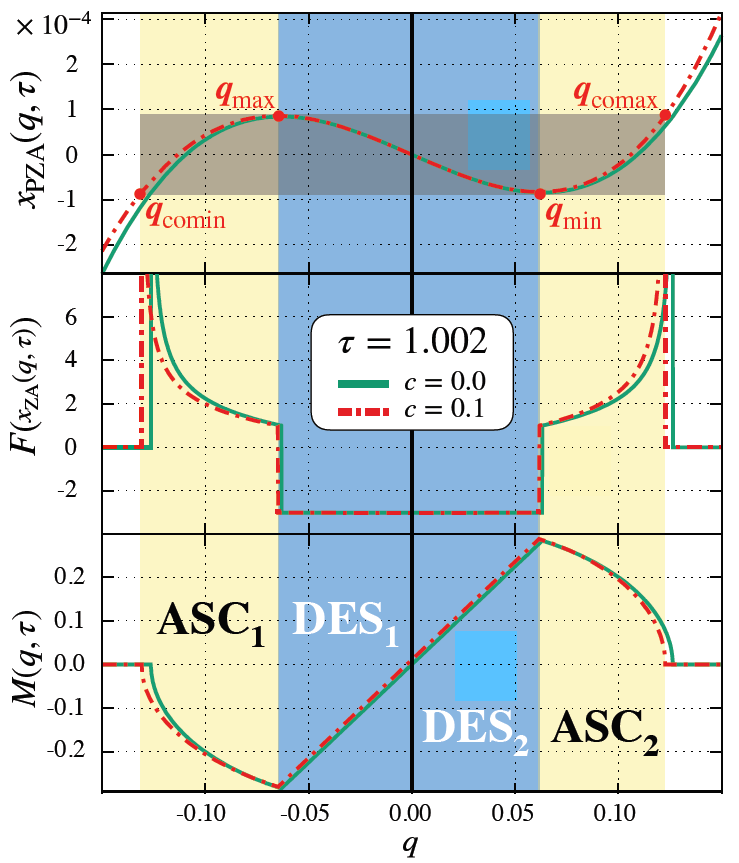
\includegraphics[scale=0.5, angle=0]{fig1.png}
        \caption{Nel pannello in alto è raffigurata un'immagine della mappa post-Zeldovich a $\tau=1.002$,
        nel pannelo centrale e quello inferiore sono mappate rispettivamente $M(q, \tau)$ e $F(q, \tau)$.
        La linea verde rappresenta la soluzione con c = 0, mentre la linea rossa tratteggiata è la soluzione
        con c = 0.1. Nel pannello in alto la zona grigia corrisponde alla zona di multistreaming, dove si
        vede che a una stessa posizione x possono corrispondere più posizioni iniziali $q$. Inoltre il primo 
        pannello definisce due regioni verticali \textit{ascending} e \textit{descending}.
        Si osserva inoltre, nel secondo pannello, la presenza di punti con derivata discontinua della forza
        generalizzata, corrispondenti a effetti di singolarità fisiche. 
        }
        \label{fig:fig1}
	\end{figure}
\end{center}

Ricavata dunque una soluzione per $\xi_c$ è possibile tornare all'equazione \ref{eqn:Sequation} 
e risolvere per $\xi_{PZA}$ utilizzando il metodo di variazione delle costanti su 
$\xi_{PZA} = \lambda(\tau)\tau + \mu(\tau)\tau^{-3/2}$ adottando le condizioni iniziali 
$\xi_{PZA}(\tau = 1) = \xi_{ZA}^{ini}$ e $\dot{\xi}_{PZA}=\xi_{ZA}^{ini}$. Su queste basi si 
ricava

\begin{equation}
    \label{eqn:finale}
    \xi_{PZA} = \xi_c(\tau) + 
    \begin{cases}
        \tau \xi_{ZA}^{ini}(q) & 0 \leq \tau \leq \tau_{com} \\
        \tau \xi_{ZA}^{ini}(q) +\frac{sign(q)}{180} \frac{D^{\frac{5}{2}}(q, \tau, c)\tau}{8-q^2+cq(48-11q^2)} & \tau_{com} \leq \tau \leq \tau_{min} \\
        -3q + \frac{4}{5}q\tau -\frac{17}{60}q^3\tau +\frac{48}{5} \sqrt{\frac{2}{2-q^2}} \frac{q}{8-q^2}\tau^{-\frac{3}{2}}+cf(q, \tau) & \tau_{min} \leq \tau
    \end{cases}
\end{equation}
d0ve la definizione di $D(q, \tau, c)$ è stata fornita in precedenza, mentre 
$f(q, \tau) = \frac{11}{20}q^4\tau -\frac{36}{5}q^4\left(\frac{2}{2-q^2}\right)^{3/2}\frac{3q^2-4}{(q^2-8)^2}\tau^{-\frac{3}{2}}$.
La \ref{eqn:finale} fornisce quindi l'andamento complessivo del dislocamento $\xi$. In figura \ref{fig:fig2} è proposto un confronto
tra previsione teorica e simulazione a N corpi.


\begin{center}
    \begin{figure}[H]
		\centering
		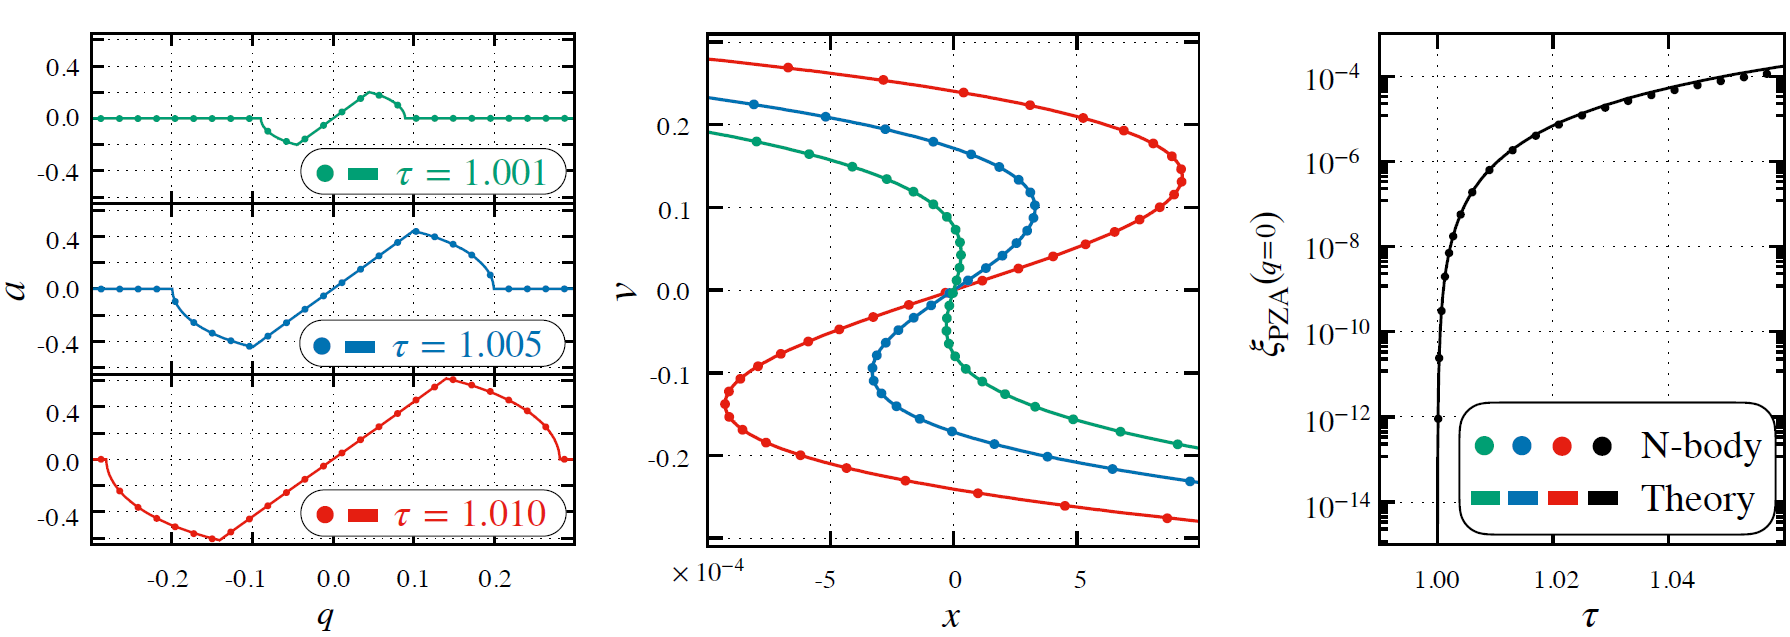
\includegraphics[scale=0.35, angle=0]{fig2.png}
        \caption{Confronto tra predizione teorica (linea continua) e simulazione a N corpi (punti).
        Il pannello di sinistra raffigura l'accelerazione $\ddot{\xi_{PZA}}$ per $c$=0, in cui è possibile 
        visualizzare alcuni punti a derivata discontinua che rivelano le singolarità fisiche, ben riprodotte 
        anche dall'andamento della simulazione. Il pannello centrale raffigura le orbite nello spazio delle fasi 
        $(x, v)$ sempre con $c$=0. Il pannello di destra invece raffigura l'improvviso valore non nullo di $\xi_{PZA}$
        al primo shell-crossing ($\tau = 1$), in conseguenza dell'attivazione della forza di multistreaming all'istante
        $\tau = 1$, costruita con $c$=0.1.
        }
        \label{fig:fig2}
	\end{figure}
\end{center}

\section{Singolarità nello spazio e nel tempo}

Nel precedente capitolo si è ottenuta infine l'equazione del dislocamento $\xi_{PZA}(q,\tau)$, definita in tre
diverse regioni temporali. Tale equazione \ref{eqn:finale} presenta delle singolarità che è possibile classificare
principalmente in due gruppi: singolarità di tipo (a), cioè quelle definite all'interno della regione temporale, e 
singolarità di tipo (b), che invece emergono quando si cerca di imporre la continuità di $\xi_{PZA}$ attraverso
le regioni di definizione. 

Una singolarità di tipo (a) si riscontra all'annullarsi della funzione $D(q, \tau, c)$, fatto che si verifica quando 
$\tau = \tau_{com}$ e se si sceglie al contempo c=0. Per investigare tal singolarità diventa necessario sviluppare
in espansione di Taylor la funzione $D$ per piccole deviazioni $\delta\tau>0$ intorno a $\tau_{com}$. Da tale espansione
si troverà che il termine dominante è del tipo $\delta\tau^{5/2}$. Un ragionamento del tutto analogo si presenta 
se l'espansione invece si compie su $q$ fissando l'istante $\tau$ ed espandendo dunque intorno a $q_{comax}$ o $q_{comin}$:
in tal caso si presenterà un termine dominante $q^{5/2}$. 


